\section{What Are Large Reasoning Models (LRMs)?}
\begin{frame}{}
    \LARGE Large Reasoning Models (LRMs)
\end{frame}

\begin{frame}[allowframebreaks]{What Are Large Reasoning Models (LRMs)?}
    \begin{itemize}
        \item \textbf{Definition:}
        \begin{itemize}
            \item Large Language Models (LLMs) optimized for \textbf{multi-step logical reasoning}
            \item Emphasize Chain-of-Thought (CoT) style reasoning
        \end{itemize}
        \vspace{1em}
        \item \textbf{Key Examples:}
        % Add a horizontal space to push the content to the right
        \hspace*{1cm}%
        % Create a minipage container that is narrower than the full width
        \begin{minipage}{\dimexpr\textwidth-1cm\relax}
            \begin{columns}[T] % Using [T] for top-alignment is good practice
                \begin{column}{0.48\linewidth} % Use \linewidth here
                    \begin{itemize}
                        \item OpenAI: o1, o3
                        \item Google: Gemini 2.0 (Flash mode)
                        \item DeepSeek: R1, V3
                    \end{itemize}
                \end{column}
                \begin{column}{0.48\linewidth} % Use \linewidth here
                    \begin{itemize}
                        \item QwQ (Alibaba)
                        \item Claude 3.5
                        \item Codestral (Mistral)
                    \end{itemize}
                \end{column}
            \end{columns}
        \end{minipage}
    \framebreak
        \item \textbf{Distinctive Behavior:}
        \begin{itemize}
            \setlength{\itemsep}{0.5em} % Adjust item spacing
            \item “Thinking internally” 
            \item Producing hidden or explicit reasoning traces
            \item Step-by-step intermediate computations
            \item Intermediate reasoning traces (explicit or latent)
            \item Better performance on symbolic tasks and math
            \item Often paired with advanced prompting or finetuning
        \end{itemize}
    \framebreak
        \item \textbf{Examples:}
        \begin{itemize}
            \setlength{\itemsep}{0.5em} 
            \item \textbf{PaLM + CoT Prompting:} \\
                Google’s PaLM + CoT prompt significantly improved accuracy on GSM8K (grade-school math) from approx 18\% to 58\%.
            \item \textbf{Gemini 2.0 Flash mode:} \\
                Provides transparent reasoning steps for decision-making.
            \item \textbf{DeepSeek R1:} \\
                Combines expert models for efficient coding and debugging. \\
                Claimed to achieve "Aha!" moments, solving reasoning tasks using structured thinking steps, not just memorization.
        \end{itemize}
    \end{itemize}

\end{frame}

\subsection{Leading Large Reasoning Models}
\begin{frame}[allowframebreaks]{Leading Large Reasoning Models}
    \large Following are some of the leading Large Reasoning Models (LRMs) as of 2024/2025:
    \vspace{0.5em}
    \begin{itemize}
        \item \textbf{OpenAI O1/O3}
        \begin{itemize}
            \item \textbf{Architecture:} Dense Transformer, RLHF-optimized.
            \item \textbf{Training Data Transparency:} Proprietary, limited details.
            \item \textbf{Strengths:} High-quality reasoning, STEM, coding.
            \item \textbf{Reasoning Approach:} Adjustable effort (Low/Med/High), step-by-step.
            \item \textbf{Efficiency:} Adjustable reasoning mode, 200K context window.
            \item \textbf{Best Use Case:} General AI, STEM research, API function calling.
        \end{itemize}
    \framebreak
        \item \textbf{DeepSeek R1}
        \begin{itemize}
            \item \textbf{Architecture:} Mixture of Experts (MoE, 671B total, 37B active).
            \item \textbf{Training Data Transparency:} Somewhat open (14.8T tokens).
            \item \textbf{Strengths:} Expert coding \& debugging, efficient MoE.
            \item \textbf{Reasoning Approach:} Multi-expert collaboration, self-improvement.
            \item \textbf{Efficiency:} High token efficiency (MoE, 312 tokens/sec).
            \item \textbf{Best Use Case:} Enterprise coding assistant, code debugging.
        \end{itemize}
    \framebreak
        \item \textbf{Gemini 2.0 (Flash Thinking)}
        \begin{itemize}
            \item \textbf{Architecture:} Multimodal Transformer (Text+Image+Speech).
            \item \textbf{Training Data Transparency:} Proprietary, multimodal (text, images, APIs).
            \item \textbf{Strengths:} Multimodal (images, text, speech), deep reasoning.
            \item \textbf{Reasoning Approach:} Flash Thinking mode (transparent thought process).
            \item \textbf{Efficiency:} 1M token context (experimental), optimized for speed.
            \item \textbf{Best Use Case:} AI assistant (multimodal, research, planning).
        \end{itemize}
    \framebreak
        \item \textbf{Claude 3.5}
        \begin{itemize}
            \item \textbf{Architecture:} Dense Transformer, fine-tuned for dialogue \& ethics.
            \item \textbf{Training Data Transparency:} Partially open (some RLHF data available).
            \item \textbf{Strengths:} Long-form dialogue, ethical AI, context memory.
            \item \textbf{Reasoning Approach:} Contextual understanding, ethical guardrails.
            \item \textbf{Efficiency:} Long context (200K), RLHF for alignment.
            \item \textbf{Best Use Case:} Long-form assistant, decision-making support.
        \end{itemize}
    \framebreak
        \item \textbf{Codestral (Mistral)}
        \begin{itemize}
            \item \textbf{Architecture:} Dense Transformer, code-focused.
            \item \textbf{Training Data Transparency:} Proprietary, open benchmarks used.
            \item \textbf{Strengths:} Cost-effective code generation, small but optimized.
            \item \textbf{Reasoning Approach:} Optimized for coding efficiency \& debugging.
            \item \textbf{Efficiency:} High speed (small model, transformer optimized).
            \item \textbf{Best Use Case:} Cost-effective coding LLM.
        \end{itemize}
    \framebreak
        \item \textbf{QwQ (Alibaba)}
        \begin{itemize}
            \item \textbf{Architecture:} Dense Transformer, fine-tuned for reasoning.
            \item \textbf{Training Data Transparency:} Limited transparency, strong math focus.
            \item \textbf{Strengths:} Math, logical puzzles, chain-of-thought self-verification.
            \item \textbf{Reasoning Approach:} Self-reflection, chain-of-thought.
            \item \textbf{Efficiency:} Small model (32B), inference-efficient.
            \item \textbf{Best Use Case:} Mathematical proofs, advanced reasoning.
        \end{itemize}
    \end{itemize}
\end{frame}


\subsection{Large language models vs. large reasoning models}
\begin{frame}[allowframebreaks]{LLMs vs. LRMs}
    \large Large language models (LLMs) and large reasoning models (LRMs) share foundational technologies but serve different purpose:
    \vspace{0.5em}
    \begin{itemize}
        \item \textbf{Core Function:}
        \begin{itemize}
            \item \textbf{LLMs:} Learn patterns in data to generate fluent, human-like text.
            \item \textbf{LRMs:} Extend LLMs to solve problems requiring logical reasoning and contextual understanding.
        \end{itemize}
        \item \textbf{Use Cases:}
        \begin{itemize}
            \item \textbf{LLMs:} Content generation, language translation, summarization, and answering user queries.
            \item \textbf{LRMs:} Math problem solving, interpreting ambiguous clinical data, and complex decision-making.
        \end{itemize}
    \framebreak
        \item \textbf{Reasoning Ability:}
        \begin{itemize}
            \item \textbf{LLMs:} Limited structured reasoning; may struggle with multi-step logic or ambiguity.
            \item \textbf{LRMs:} Trained to apply consistent reasoning steps; outputs are more logical and verifiable.
        \end{itemize}
        \item \textbf{Performance:}
        \begin{itemize}
            \item \textbf{LLMs:} Fast response times; optimized for scalability and speed.
            \item \textbf{LRMs:} Slower response times; require more processing to reason through problems step by step.
        \end{itemize}
        \item \textbf{Best Suited For:}
        \begin{itemize}
            \item \textbf{LLMs:} High-volume, low-risk tasks where speed is critical.
            \item \textbf{LRMs:} High-stakes or complex tasks where accuracy, explainability, and logic matter.
        \end{itemize}
    \end{itemize}
\end{frame}


\subsection{How Do LRMs Work?}
\begin{frame}[allowframebreaks]{How Do LRMs Work?}
    \begin{center}
        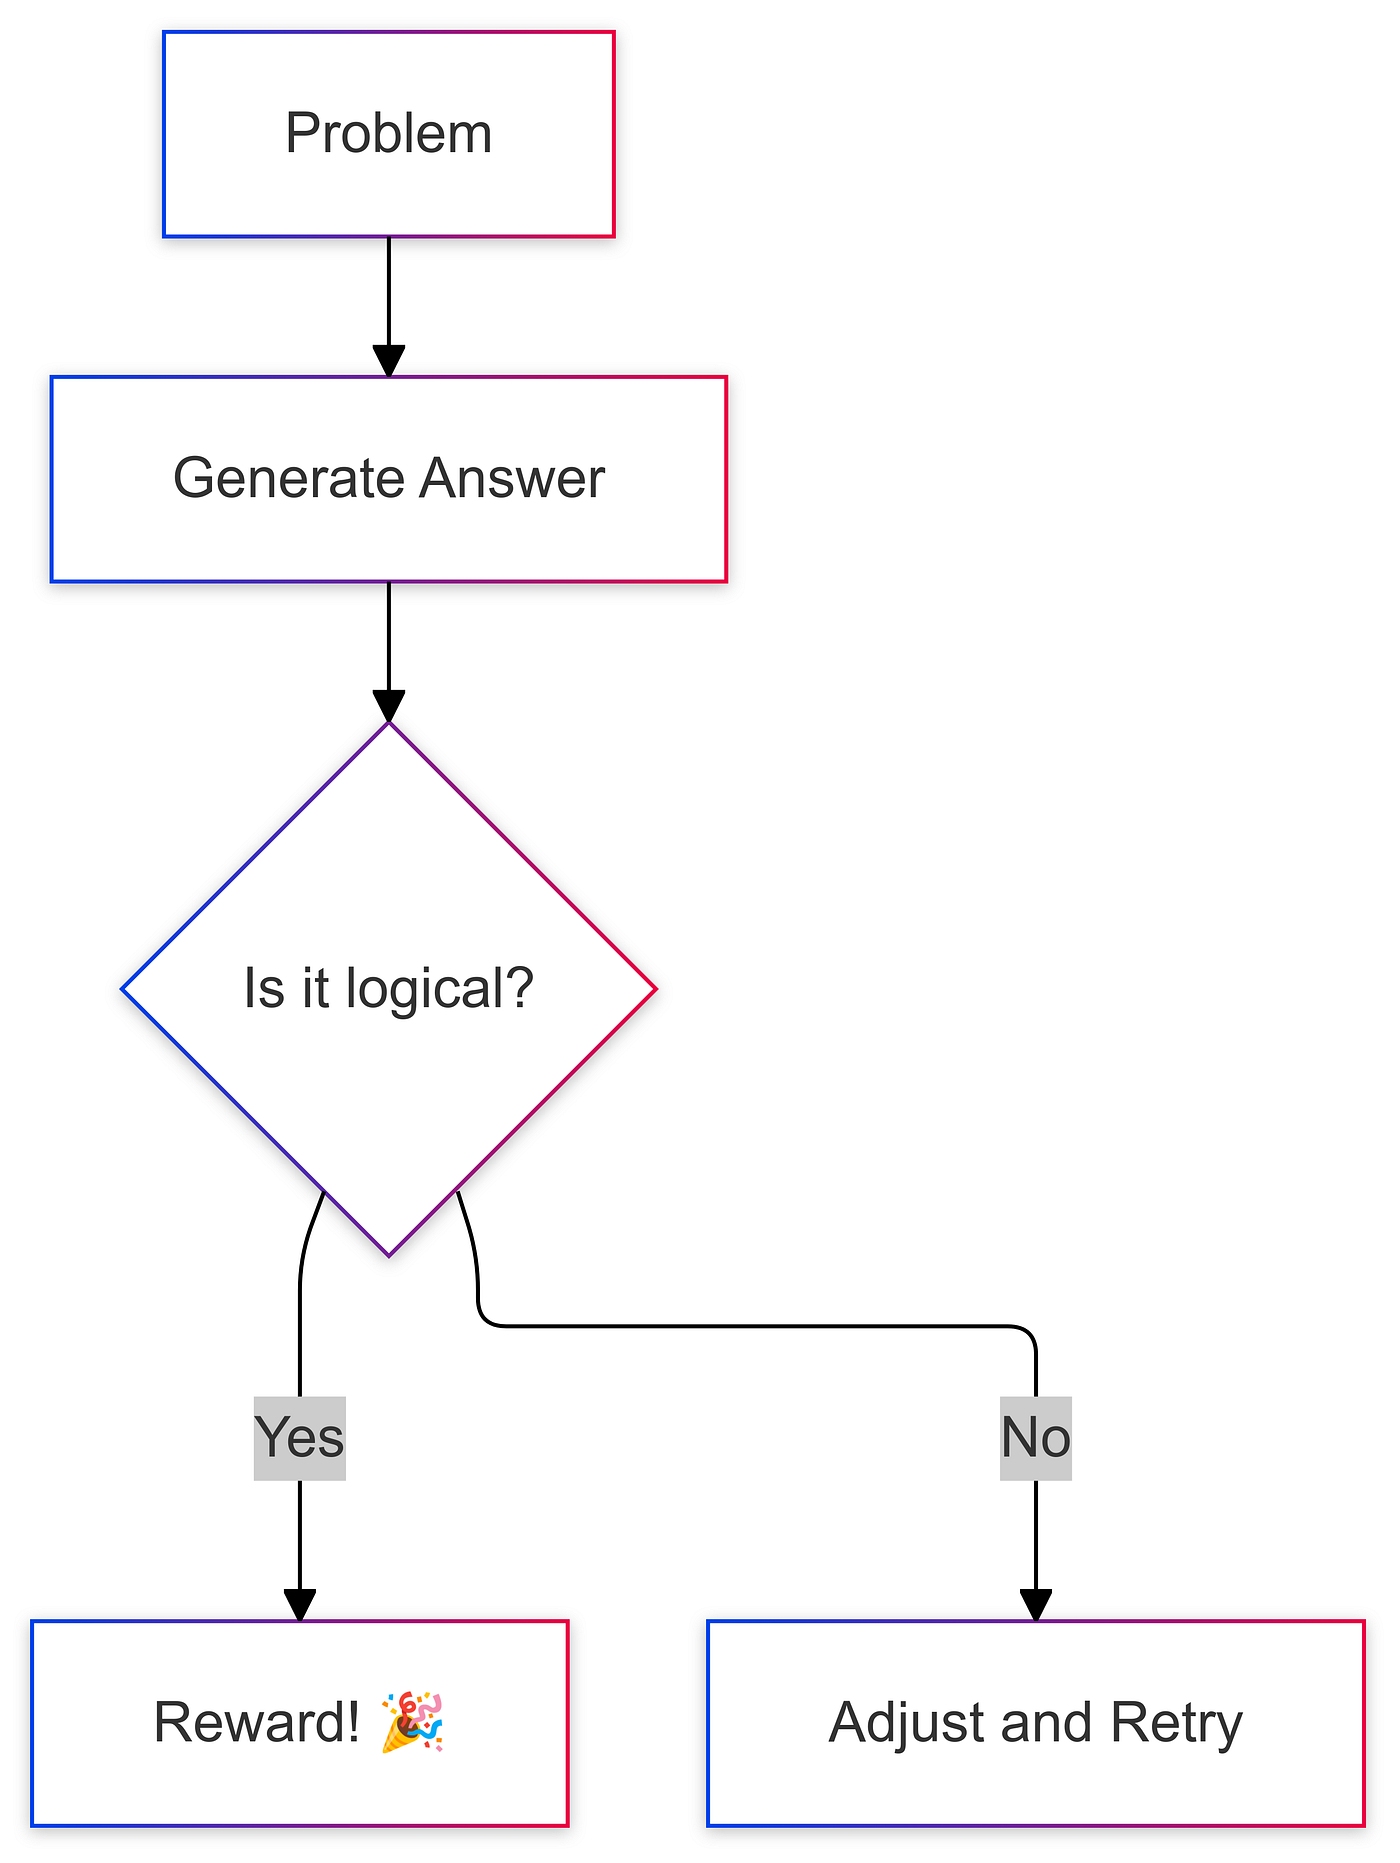
\includegraphics[height=0.9\textheight, width=\textwidth, keepaspectratio]{images/lrm+moe/lrm-2.png}
    \end{center}
\framebreak
    LRMs use a combination of training methods and prompt strategies to enhance the reasoning capabilities of LLMs. 
    \vspace{0.5em}
    \begin{itemize}
        \item \textbf{Training on Enriched Datasets}
        \begin{itemize}
            \item Includes reasoning-focused examples
            \item Real-world scenarios with clear outcomes
            \item Teaches both correct answers and reasoning steps
        \end{itemize}
        \item \textbf{Reinforcement Learning (RL)}
        \begin{itemize}
            \item Rewards for logical, correct answers
            \item Penalties for incorrect or inconsistent reasoning
            \item Reinforces desirable reasoning patterns
        \end{itemize}
        \item \textbf{Human Feedback (RLHF)}
        \begin{itemize}
            \item Human reviewers guide model outputs
            \item Refines nuanced reasoning strategies
            \item Useful in domains needing expertise (e.g., healthcare, finance)
        \end{itemize}
        \item \textbf{Prompt Engineering}
        \begin{itemize}
            \item Carefully designed prompts activate reasoning
            \item Guides model through multi-step or layered tasks
            \item Generic prompts may not trigger deep reasoning
        \end{itemize}
        \item \textbf{Chain-of-Thought (CoT) Prompting}
        \begin{itemize}
            \item Breaks problems into smaller steps
            \item Explores multiple reasoning paths
            \item Improves transparency and accuracy
            \item Essential for auditability and explainability
        \end{itemize}
    \end{itemize}
\end{frame}


\subsection{Types of reasoning in LRMs}
\begin{frame}[allowframebreaks]{Types of Reasoning in LRMs}
    Large reasoning models (LRMs) employ several types of reasoning to simulate or support human-like problem solving:
    \vspace{0.5em}
    \begin{itemize}
        \item \textbf{Deductive Reasoning}
        \begin{itemize}
            \item Applies general rules to specific cases for logically certain conclusions (top-down reasoning).
            \item Excels at structured, rule-based tasks requiring high logical consistency.
            \item Example domains: regulatory compliance, medical protocol analysis.
            \item \textit{Example:} \\
            \textbf{Rule:} All patients with a fever and cough should be tested for influenza. \\
            \textbf{Case:} Patient A has a fever and cough. \\
            \textbf{Deduction:} Patient A should be tested for influenza.
        \end{itemize}
    \framebreak
        \item \textbf{Inductive Reasoning}
        \begin{itemize}
            \item Draws general conclusions from specific observations in data.
            \item Supports probabilistic predictions and generalization to unseen inputs.
            \item Useful in dynamic, data-rich scenarios (e.g., fraud detection).
            \item \textit{Example:} \\
            \textbf{Observation:} 90\% of emails with suspicious links are phishing attempts. \\
            \textbf{Induction:} An email with a suspicious link is likely to be a phishing attempt.
        \end{itemize}
    \framebreak
        \item \textbf{Abductive Reasoning}
        \begin{itemize}
            \item Infers the most likely explanation from incomplete or uncertain evidence.
            \item Generates hypotheses rather than definitive answers.
            \item Effective in domains like medical diagnostics, where plausible interpretations are needed.
            \item \textit{Example:} \\
            \textbf{Evidence:} The lawn is wet in the morning. \\
            \textbf{Possible explanations:} It rained overnight, or the sprinkler was on. \\
            \textbf{Abduction:} If the weather report says no rain, the most likely explanation is the sprinkler was on.
        \end{itemize}
    \framebreak
        \item \textbf{Analogical Reasoning}
        \begin{itemize}
            \item Identifies similarities between different situations or datasets.
            \item Transfers insights from one context to another for novel problem solving.
            \item Example: recommending products based on similar customer behavior.
            \item \textit{Example:} \\
            \textbf{Situation A:} A student learns to solve quadratic equations by factoring. \\
            \textbf{Situation B:} The student applies the same factoring method to solve cubic equations. \\
            \textbf{Analogy:} The approach used for quadratics is adapted to cubics.
        \end{itemize}
    \end{itemize}
\end{frame}